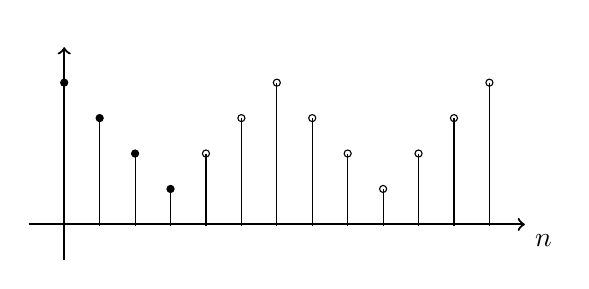
\begin{tikzpicture}[scale=0.45]
    \draw[thick,->] (-1,0) -- (13,0) node[anchor=north west] {$n$};
    \foreach \x in {1,...,12}
        \draw (\x cm,1pt) -- (\x cm,-1pt) node[anchor=north] {};% {$\x$};
    \draw[thick,->] (0,-1) -- (0,5) node[anchor=south east] {};
    
    \foreach \x in {0,...,3} {
        \filldraw[fill=black, draw=black] (\x cm,4-\x) circle (0.1cm);
        \draw (\x,4-\x) -- (\x,0);
    }

    \foreach \x in {4,...,6} {
        \draw[draw=black] (\x cm,\x-2) circle (0.1cm);
        \draw (\x,\x-2) -- (\x,0);
    }

    \foreach \x in {7,...,9} {
        \draw[draw=black] (\x cm,4-\x+6) circle (0.1cm);
        \draw (\x, 4-\x+6) -- (\x,0);
    }

    \foreach \x in {10,...,12} {
        \draw[draw=black] (\x cm,\x-8) circle (0.1cm);
        \draw (\x, \x-8) -- (\x,0);
    }
\end{tikzpicture}